 % This is an example LaTeX document showing how to use the l3proj class to
% write your report. Use pdflatex and bibtex to process the file, creating 
% a PDF file as output (there is no need to use dvips when using pdflatex).

% Modified 

\documentclass{l3proj}
\usepackage{graphicx}
\usepackage{float}
\begin{document}
\title{Remote Performance Monitoring Using Websockets}
\author{Maksim Solovjov \\
        Aleksandrs Sidlovskis \\
        Sean Jakobsen \\
        Gabriel Alexandru Susanu \\
        Supanat Auengsirirat}
\date{16 March 2014}
\maketitle
\begin{abstract}

The goal of this project is to create a web application that allows users in or outside of the Univeristy of Glasgow to monitor the performance of their servers remotely and in real time. Our application consists of a web client to be used inside a browser, a server written in Go - currently hosted ourselves - and daemons that the user will install on any and all machines they wish to monitor.

\end{abstract}
\educationalconsent
\tableofcontents

%===============================================================================================================================================

%===============================================================================================================================================

\chapter{Preliminaries}
\label{prelim}

(THIS IS A GLOSSARY, WHICH SHOULD BE AN APPENDIX)

Here are the necessary terms that a reader may not be familiar with. More knowledgeable readers may feel free to skip this section of the report.

\textbf{Performance monitoring} – observing the statistics of some system, which relate to how well the system runs. For example monitoring the CPU load in order to ensure that it does not exceed some healthy threshold.

\textbf{Cloud-based solution} – the program that is provided as a service on some external machines (which might be owned by a separate organisation) accessible via internet.

\textbf{Client (Application)} – in our case, a user-facing application, running in a user’s browser.

\textbf{Server} – a computation-intensive application that serves the client application to the user and provides the gateway to the database.

\textbf{Daemon} – a monitoring application, running on the machine that is to be monitored, storing the performance metrics and sending them to the Server and Client.

\textbf{Relational database} – a database, modelled by creating entities and expressing their relationships to each other. Interaction with the stored data is governed by relational algebra.

\textbf{NoSQL database} – an alternative to the relational database, which allows easy horizontal scaling (can accommodate more data), in our case (MongoDB) expressed via collections of documents with no enforced schema (blueprint).

\textbf{WebSocket} – a protocol, that allows simultaneous bidirectional communication over a single TCP connection. To put it in simple terms, it lets a user to both send and receive data in real-time without the overhead of making multiple ``internet'' connections.

\textbf{Concurrency} – splitting work into independent chunks, that can be done in any particular order, allowing switching from one task to another should the first one temporarily stall.

\textbf{Parallelism} – executing multiple concurrent tasks at the same time. 

\textbf{Refactor} – rewrite, in order to improve the quality of the code without changing its output.

%===============================================================================================================================================

%===============================================================================================================================================

\chapter{Introduction}
\label{intro}

This team is comprised of five members from the University of Glasgow's Software Engineering course. We have been given two semesters to work on a project as part of our coursework and this document outlines the results of our work.

(MENTION THAT THE PROJECT WAS PROPOSED BY J.P.MORGAN)

\section{Motivation}
\label{motivation}

(YOU COULD TALK ABOUT SECTOR EXPECTATION OF GROWTH (MOORE'S LAW) AND SOCIETAL DEMAND FOR GROWTH (BIG DATA))

As computing power grows, so do our ambitions, which, in turn, require even more computing power to satisfy. Quite often, this cycle forces companies to deploy huge datacentres filled with machines. (GIVE QUANTITATIVE EXAMPLE - MS SAY THEY HAVE 1 MILLION SERVERS ACROSS THEIR DATACENTRES - GOOGLE FOR ``MICROSOSFT NOW HAS ONE MILLION SERVERS'' - MID 2013) But this necessary show of force poses many problems, one of particular importance being how to ensure the whole infrastructure runs smoothly.

The key step in any managed solution, be it automated or manual, is to monitor how the system is performing. A multitude of different parameters might be used to express the performance; however, for most systems it is enough to know:

\begin{itemize}
  \item CPU load
  \item Network load
  \item Memory usage
  \item Temperature
  \item Memory usage
  \item Accessibility of the system
\end{itemize}

This data should be available in real-time, since otherwise there is an artificial delay in how quickly one can respond to the emerging problem. Finally, the installation of such a system should be as easy as possible, since there are many other things that system administrators already have to setup, and our aim is to make their life easier.


\section{Aims}
\label{aims}

While not unique --- many solutions for server monitoring already exist - this project offers a chance for innovation and creativity in the space. We cannot compete with features in the time we have or with the size of our team, we hope to improve on usability and target a user base of people who just don’t need or want the complexity of our competitors. During market research we discovered that our competition monitors hundreds of metrics and statistics, and as a result the interfaces are extremely cluttered and confusing. Also, not many promoted real-time data monitoring, so this could really set us apart from some of the market leaders and make our solution a viable product.

To reiterate, should our project meet our aims of:

(BE MORE SPECIFIC)

\begin{itemize}
  \item Simplicity
  \item Legibility
  \item Usability
  \item Real time feedback
\end{itemize}

Then we can deem it a success.

%===============================================================================================================================================

%===============================================================================================================================================

\chapter{Background}
\label{background}

\section{The Problem}
\label{section:problem}

%Initial problem description,

Taken from the list of this year's team project descriptions:

\begin{quotation}
A generic performance metric gathering tool would allow systems to easily send in metric data (e.g. CPU utilization). This would allow sysadmins to monitor processing speed (units of work per second) over time and spot trends.

HTML5 technologies are increasing in popularity and providing alternatives to third party browser plug-ins such as Flash for providing interactive, immersive, real time web applications. Among these innovations are Web Sockets and Javascript based charting.
Web Sockets provide full duplex client-server messaging with initiation through HTTP. With its lower overhead than comparable techniques such as Comet and Ajax Long Polling this promises to make web applications truly real time with servers able to push new data to client browsers in an ad-hoc / ``as it arrives'' fashion.

Web Sockets would allow a server-side performance metrics storage system to push newly arriving performance data to a web browser based console.

This system will allow other systems to add performance metrics and allow users to view tables and charts through the browser without need for third party plug-ins. Investigation should take place to evaluate if Web Sockets would be performant enough to deliver this information in real-time and update charting without refreshing the page.
\end{quotation}

\section{Our Interpretation}

%How we understood the problem

From the problem description in Section ~\ref{section:problem} we understood the problem to be a case of monitoring system level metrics and allowing a user to view these statistics remotely. Moreover, there is emphasis on utilising web sockets for their ability to send and receive data in real time, indeed, this would be the ultimate focus of our solution: real time performance monitoring.

\section{Market Research}
\label{section:MarketResearch}

%A study of existing solutions

(YOU NEED TO DO A PROPER SURVEY - COMPARE \& CONTRAST THEIR FEATURES. HAVE SCREENSHOTS, URLS, LISTS OF FEATURES)

Our goal to create a system that allows for the monitoring of real time server system data is not unique. In fact several well established companies are already doing much of what we want to and, on occasion, do so on a scale multiple times that of which we initially thought our own could be. Looking into these competitors has refined what we hope to achieve with our own system, grounded our expectations and will hopefully fuel creativity.

\textbf{What should we monitor?}

Our competition offer literally hundreds of processes, events and hardware statuses to be monitored, some even offering hardware sensors that can be installed to monitor the climate in the client’s server control room. While these are fun to think about, it quickly became apparent that this was a bullet point we simply could not compete with. Instead, we should focus primarily on gathering the most useful and relevant data that we can such as CPU data, memory stats, traffic etc as outlined in Section \ref{motivation}. We still have the potential problem of handling multiple operating systems, so biting off more than we chew is a real possibility otherwise.

\textbf{Competition has complicated interfaces}

Monitoring less stats also allows us the opportunity to really improve a feature that so many people seem to overcomplicate, UI. Offering so many things in one package makes our competition seem very bulky, non-intuitive and threatening. Lists upon lists upon graphs upon menus are displayed side by side and it seems a far from ideal layout. By working with the simplest data that the user needs, there is an opportunity for us to display graphs, allow for manipulation and offer customisation while still keeping this important information available at a glance, not hidden between tabs or scrolling panes.

\textbf{We should be able to set up alerts}

A common feature among similar products is the ability to set up custom alerts for specific data. Say the memory reached capacity and could have a potential knock-on effect to a company’s customers, an alert could be set up so that memory was monitored and an email would be sent to the system admin (most likely via email) if it reaches a certain threshold. This also emphasises how critical it can be to have access to a server’s system data with as little latency as possible and is an ideal addition to fulfill our brief.

\textbf{Predicting, preventing and repairing failures automatically is beyond us}

A more complex issue that links into the idea of alerts would be the ability for us to detect failures and problems without custom scripts or alerts. Many systems offer this functionality and some even promote their ability to repair failures automatically, however, this is beyond our own project.

\textbf{Potential for guidance if not automatic action}

One system had a review stating that many performance counters gave a definition of the metric, an explanation of what the possible problem may be and suggestions of how to remedy the issue. With our system aiming at smaller set ups, it’s very likely that our user base will consist of novices, and such a feature could be highly useful. This of course presents the problem of showing information when it is needed to users who may not know about it, while also preventing it from becoming a nuisance, or making it hideable to experts.

(TOO VAGUE)

\textbf{Closest competition has poor refresh rate}

Our seemingly closest competitor is a free solution that boasts a refresh rate of 30 minutes, it’s premium flavour reducing that to 1 or 5 minutes depending on how it is set up. Also boasting simplicity, it could be one to dig into more closely in order to discover how it handles its interface, a one dashboard view.

\textbf{We should promote simplicity at all stages}

Promoting simplicity and usability is definitely our main goal and so our solution should be just as easy to set up as it to work with. A short install time is something we will definitely be aiming for.

%===============================================================================================================================================

%===============================================================================================================================================

\chapter{Requirements}
\label{req}

From team discussions, as well as our market research, we constructed a list of requirements to be fulfilled during the progress of this project.

(LABEL EACH REQUIREMENT. PRIORITISE EACH REQUIREMENT)

\section{Functional Requirements}

%Requirements discovered that focus on a user's interaction with the saystem

\subsection{Requirements Table}

\subsection{Use Case Diagrams}

\subsection{User Requirements Details}

\section{Non-Functional Requirements}

%Requirements discovered that focus on how the system should perform while being used

\subsection{Server Requirements}

The emphasis for the server is on the horizontal scalability. It has to provide concurrent access for multiple users from multiple organisations to multiple daemons. In order to make this requirement testable, we have decided to translate it to the following numerical equivalent:
\begin{enumerate}
\item it has to support 1000 concurrent users,
\item belonging to 100 different organisations,
\item monitoring 10000 different daemons.
\end{enumerate}

We feel that these requirements outline a reasonable scenario describing a moderate usage by a hundred middle-sized companies. The server must support them while still running on a single machine, otherwise the server should probably be deployed on an elastic cloud, rather than a single PC.

\subsection{Daemon Requirements}

Due to the fact that the daemon is meant to run constantly in the background on monitored machines, the focus was on keeping it small and very fast while providing all the required monitoring and communication features.
Furthermore, due to the variety of platforms clients would like to monitor, the daemon must be easy to deploy and develop for most platforms.
Internally, the daemon needs to send data regarding all the monitored paramters to our central server, as well as all clients that are currently connected to it for real-time data gathering.
To do this, the daemon has to implement a common communication protocol, initiate a connection to the server, and accept any number of connections from clients.


Gabriel - how does daemon sending data affect the performance of the system it's running on. Remember you ran some tests to see how big of an impact this was? Can talk about how the daemons perform in our evaluation, but how did we deem what would be acceptable?

%===============================================================================================================================================

%===============================================================================================================================================

\chapter{Design}
\label{design}

(HAVE AN INTRODUCTORY `SIGNPOST' PARAGRAPH AT START OF EACH CHAPTER.)

%-----------------------------------------------------------------------------------------------------------------------------------------------

\section{Overall system}

\subsection{High level design}

We decided that the best way to tackle this problem was to split it into three main components and a database:

\begin{figure}[H]
\centering
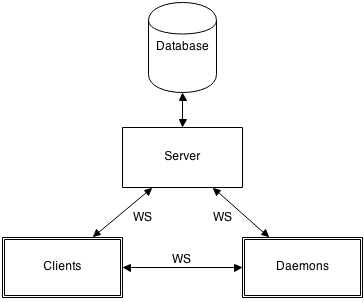
\includegraphics[width=110mm]{images/ArchitectureDiagram.png}
\caption{Architecture Diagram}
\end{figure}

(MORE SPECIFIC CAPTION)

At the center we have a single web Server. It acts as a broker between the Client and the Daemon in order for them to establish a connection, as well as storing historical monitoring data that the Daemon sends. All the control messages that the Client might want to issue to the Daemon will also go through the Server.

(WHAT IS A CLIENT? EXPLAIN HERE)

A Server can support multiple Clients and Daemons communicating at the same time. They will be organised in the organisations they belong to, more on that later.

The client is a web application that shows real time performance data from the Daemons. In order to do so, it directly establishes a websocket connection to one or many Daemons, with the help of Server. It can also retrieve historical data for any given Daemon that it has access to from the Database through the Server.

A Daemon is a small application that runs on the machine and monitors its performance. It sends the data that it gathers to one or many Clients in real time using websockets, and it also stores sparser data points in the Database through the Server. It can be told to monitor different things, and these commands come through the Server.

Such separation of concerns flows naturally from the description of the task. It also enables us as a team to develop multiple independent parts in parallel.

A key to success in this case is the communication API. All three components implement the fully documented API, which ensures painless integration of the components, as long as the API is developed before them.

\subsection{The Technology}

The Client is a web-based application written in HTML5, CSS3, and CoffeeScript. The libraries used are Backbone.js, Marionette.js, jQuery, Chart.js and Bootstrap.

The Server runs on Linux and is written in Go. It uses a MongoDB database for storing the data.

Daemon can be compiled to target multiple platforms and is written in C++.

\subsection{Motivation For The Choice Of Technologies}

(GIVE REFERENCES --- MAYBE URLS OR ARTICLES?)

\textbf{HTML5} is the most modern standard for a markup language which is supported by a huge number of web browsers. This is the de facto standard technology, and hence a sensible choice.

\textbf{CSS3} is a style sheet language that is used to describe the look of the document. Much like HTML5, it is a standard for the modern Web. At first we thought about using LESS (which in turn would be compiled to CSS) as it introduces some nice features like variables, nesting, loops and functions. However, due to the fact that there would most likely be more negatives than positives when introducing a language not many were familiar with, it was decided to stick with the standard.

\textbf{CoffeeScript} is a language that compiles to JavaScript. The main motivation to use it was the opportunity to learn something new. It adds some syntactic sugar to JavaScript which greatly improves the speed of development. Some of the team members started to use CoffeeScript in their daily development tasks.

\textbf{Backbone.js} is a model-view-presentation framework for front-end development. Together with Marionette it gives a very simple way to build large client-side applications. This framework was ideal for us, as it offers a huge number of features for single-paged apps. Similar to CoffeeScript, choosing this framework was motivated by an opportunity to learn a new programming paradigm and expand our toolkit.

\textbf{jQuery} is a library that massively increases the speed of web development. We can not even imagine developing a large application without using this as it offers an enormous amount of useful shortcuts. Many team members know from experience that working with DOM directly always takes much more time than using jQuery. Also, it minimizes the differences of browser behaviours.

\textbf{Chart.js} is a library that is great in drawing data-driven charts. In our case it is responsible for presenting all the graphical information.

\textbf{Bootstrap} gives us a fast way to make the application look similar on every platform. Also, it makes the user interface absolutely platfom-independent, both on mobile and desktop devices.

\textbf{Go} was chosen for its potential to scale horizontaly. It has an extremely nice concurrency based on goroutines, which are sort of managed lightweight threads. It also features extremely fast compilation times, serving as a boost to development speed. Additionally, even though it is statically typed, it has a runtime that allows easy type assertion, and garbage collection, making writing Go almost as fast as using scripting languages (for those who know Go). Its closest opponent was Rust, which is a much more linguistically exciting language, but we decided to refrain from using it, seeing it as less mature.

\textbf{MongoDB} is a NoSQL database, which was once again chosen due to its immense horizontal scaling abilities. It is relatively mature at this point with an ever increasing online community and good documentation, thus it seemed to be a fair choice, knowing that we will have vast amounts of loosely structured data to deal with.

%-----------------------------------------------------------------------------------------------------------------------------------------------

\section{Client Application}

\subsection{Goal}

The web application has to provide an intuitive way of viewing how the remote machines are using their resources. The client does not have to know anything about the monitored machine - he/she just needs to see the information about it. The user interface should provide an opportunity to display this information in real time as well as the history of usage for a specified period of time.

On top of this data-centric display, the application should be capable of providing some implicit information. For example, if the daemon does not appear in the list of registered daemons, or it states that it is not active at the moment, the user should know somehow in order to check if the machine is running correctly, or if it has an internet connection. One useful feature of the system would be the ability to send alerts to the user, an alert popping up whenever an abnormal activity is detected, most likely this could be implemented as an automated email. The application must also provide an easy process of new user and daemon registration, with users potentially neeind to perform this operation multiple times.


\subsection{Flow}

All the client-server and client-daemon communications are done through WebSocket messages. A single HTTP GET request is sent to receive the application and from there, once the user interface is loaded, a single, self-restoring, WebSocket connection with the server is established. As the WebSocket API provides a method ``onclose'', we will know if and when the connection is lost. In this case a timer is created and after a short timeout a new connection attempt is made.

Once a client-server connection is established, the user implicitly sends a ``login'' check message that contains a ``session id'' cookie. The server can respond with two kinds of answers. The first one is an ``error'' message, that indicates that the server does not have any information about the cookie provided or that the session has already expired. In this case the application answers by changing the current view to the login page. Another answer indicates that the user is logged in. In this case the current view is changed to the home view of the application.

The login screen is just a standard form with login and password fields. When the required information is provided, a message to the server is sent. If the password matches the specified user name, the user receives a new cookie and some more information about himself and the view is changed to the home view. On error, the login page remains, with some message to the user saying that their login attempt failed.

After a succesful authorization (cookie or login), a ``daemons'' request is sent, the answer to this request being a list of daemons associated with a requesting user. Every element of the list contains some basic information about a daemon and to get more specific information the user should send another request called ``daemon'' including this daemon's ID. The reply to this request is simply a list of further information, including the address, specific to the desired daemon. When the address of a daemon is received, the connection is made instantly and the real-time monitoring data is sent to the client. Now on every incoming message the corresponding data chart is refreshed to show the actual resource usage.

\subsection{UML}

The UML diagram showing the design on the client will be here.

\subsection{Components}

As we are using Backbone which is a model–view–presenter (MVP) framework, the code is very nicely structured. Every component is a separate file written in CoffeeScript.

All the components can be split in groups:
\begin{itemize}
  \item UI components (views for tabs, daemons, charts, alerts)
  \item Model components (tabs, daemons, charts, alerts)
  \item Controlling component (controller.coffee - high-level callbacks and the daemon object)
  \item Service component (service.coffee)
  \item Framework specific components (Router, AppState)
  \item Communication component (Messages, Message Processor and Sockets)
\end{itemize}

\subsection{Concept Designs}

Prototyping our user interface was an obvious task before doubling down on development. With the user experience such a prominent focus to the team, this would enable us to put ideas down on paper very quickly and inexpensively in order to achieve a clear and singular design vision in everyone's minds before proper development started. If executed properly, these designs should fulfill our user requirements of simplicity and usabilty, while also making development more focused and planned out.

When considering what would have to be evaluated with these designs, the primary goals were to:

Show appropriate information without crowding the page

Allow a user to navigate easily

Provide functionality deemed necessary from (MARKET RESEARCH, OTHER SECTIONS...)

When discussing these designs, the motives behind certain decisions will be explored alongside the proposed outcomes. This should build upon and solidify any of the requirements as specified in Section (REQUIREMENTS SECTION).

\begin{figure}[H]
\centering
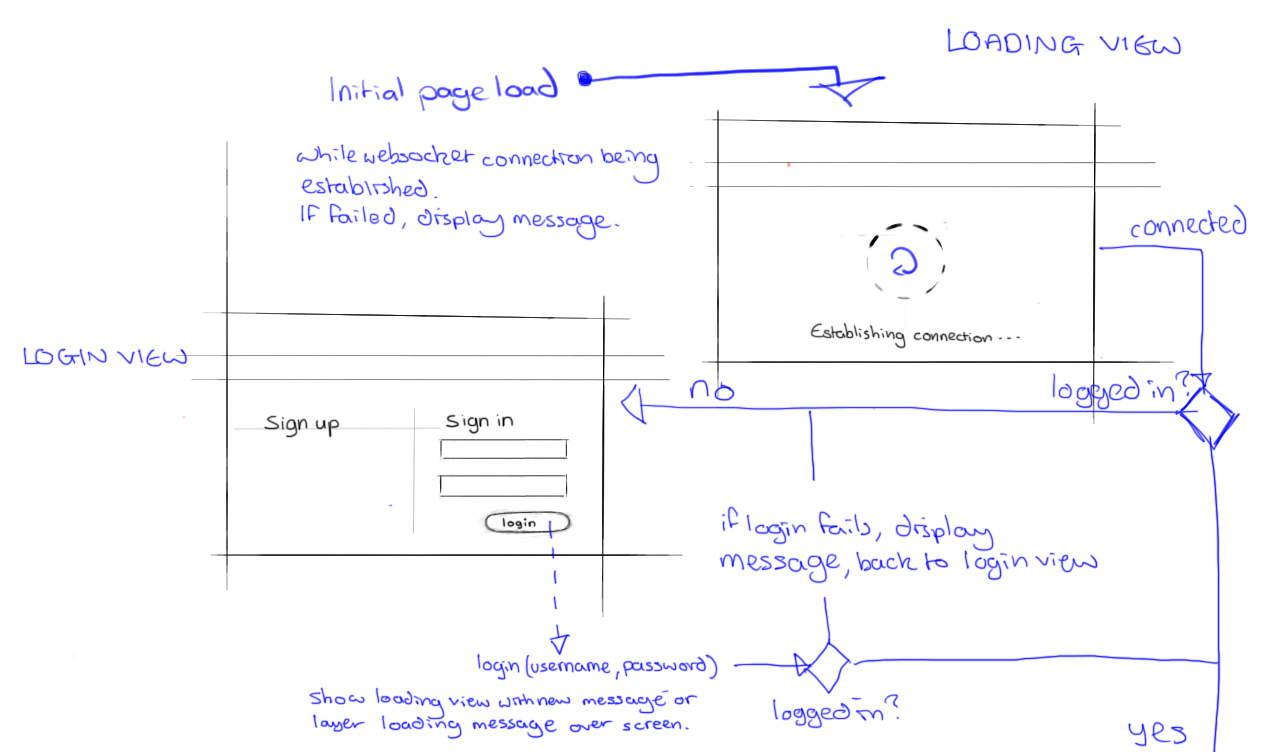
\includegraphics[width=110mm]{Concept_Designs/Login.png}
\caption{Login screen}
\label{fig:Login}
\end{figure}

The login screen shown in Figure \ref{fig:Login} should remain simplistic, and upon full completion may include some basic information about the project as a form of publicity or advertisement. However, the main feature explored here is simply the client's ability to establish a connection with our server.  With this project relying so heavily on information gleamed from the cloud, the user would have to be notified when the server was working to provide this information, while there was nothing to see yet. So, on the login screen, while a connection is being established, a spinner could be used with a simple message to keep the user informed of what's happening and why there may be any delay. This is a nod to the helpful and friendly user experien we aim to provide throughout the rest of the application.

In Figure \ref{fig:MainDash} you can see this spinner returning to inform the user that information is being accessed from the server, and there is currently nothing to see.  Obviously, any 'loading' times should be reduced to an absolute minimum, but designing for the worst case scenarios and keeping them in-line with our best-case visions will hopefully unify the application and make it seem more professional, even when it stutters or fails.

\begin{figure}[H]
\centering
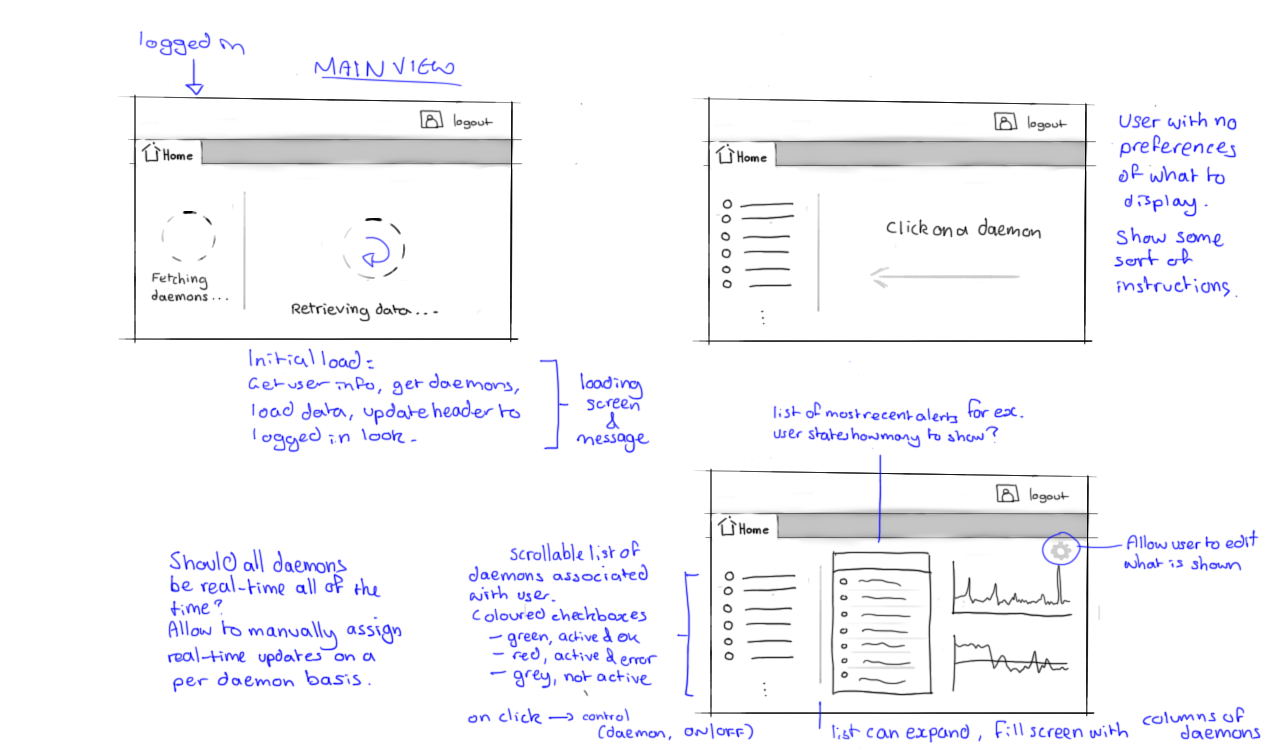
\includegraphics[width=110mm]{Concept_Designs/MainView.png}
\caption{Main Dashboard}
\label{fig:MainDash}
\end{figure}

To focus on some of the functionality now, there is a list of Daemons (installed on the user's servers) on the left side of the screen and a navbar at the top of the screen. These will remain constant once a user has logged in, allowing for a kind of visual anchor or safety net. As they navigate to different parts of the app, the header and sidebar should never really change much, so the user should not have to search around or relearn the interface when they switch between creating an alert or simply viewing the latest graphical data of a selected Daemon. This was developed from our requirement of designing an app that is simple and clean.

The rest of the screen can be described as a content area.  Here, in the main dashboard, the initial idea was to allow for a user configurable space, where the user would choose what they wanted to see as soon as they logged in. In the bottom-right of Figure \ref{fig:MainDash} you can see an example layout where the user wishes to see a list of the most recent alerts for any selected daemon, along with two chart views of some metrics (perhaps CPU usage and network traffic). Again, this was developed as a counter to competitors' cluttered dashboards where one may get lost in before they found what they wanted. This way a user could access their own most useful stats as soon as they logged in.

Now, let's say that a user has just installed Daemons on their machine(s) for the first time, and are now logging in. The top-right of Figure \ref{fig:MainDash} shows this scenario being played out, with the content panel now providing instructions to the user on how to get started. Indeed, simply installing the Daemons will not mean there is an instant connection to those machines and the client's interface in the final product. We have to provide some way of notifying the user that a Daemon is not currently active. The solution is to colour code our daemon list, with grey icons representing inactive daemons that a user can click on to 'turn on'. Similarly, green icons represent active daemons that are running without problem, and red icons represent daemons that are active but have encountered some kind of error, or the system they are running on is performing poorly. This information should help provide context to the user at a glance and allow them to make appropriate decisions quickly and easily.

\begin{figure}[H]
\centering
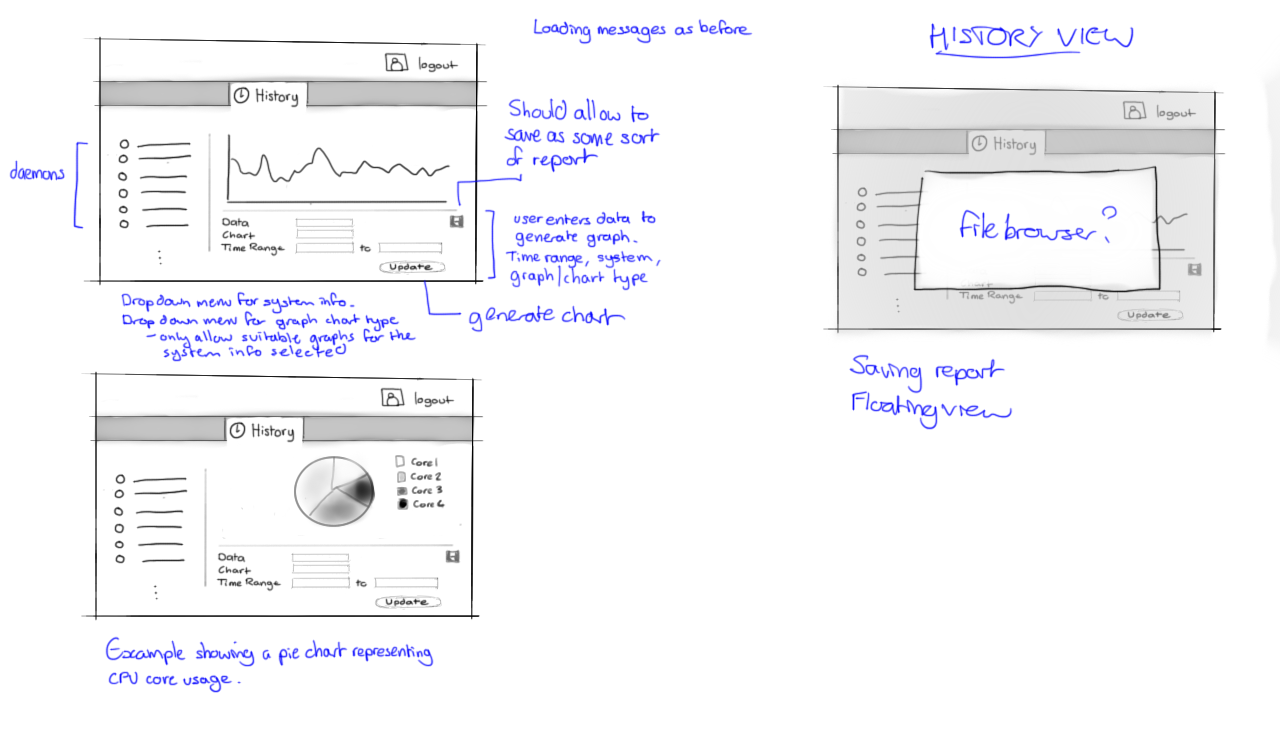
\includegraphics[width=110mm]{Concept_Designs/HistoryView.png}
\caption{History View}
\label{fig:HistoryView}
\end{figure}

When a user wishes to view past data stored in the server's database, they would click on the History tab. Notice how now, in Figure \ref{fig:HistoryView}, the header has changed to highlight the selected tab, so it is clear to the user where they are in the application. Also, the content panel has now changed to provide the functionality for this specific tab. Like before, a user selects the daemon they wish to query from the left sidebar, and then in the content view they can specify a specific metric's history to view as well as a time-range.

Now with our project being part of our university coursework, this will likely be a free and open-source solution, and as such storing data indefinitely is completely unreasonable. Over time, the resolution of a user's past data is decreased in order to make room for high resolution recent data. But rather than just deleting old data and leaving it at that, it was decided that a user should be able to save a historical view of a daemon's data. In this history tab is a save icon to allow the user to do just that, perhaps bringing up a file browser for more control over what happens with the generated file.

\begin{figure}[H]
\centering
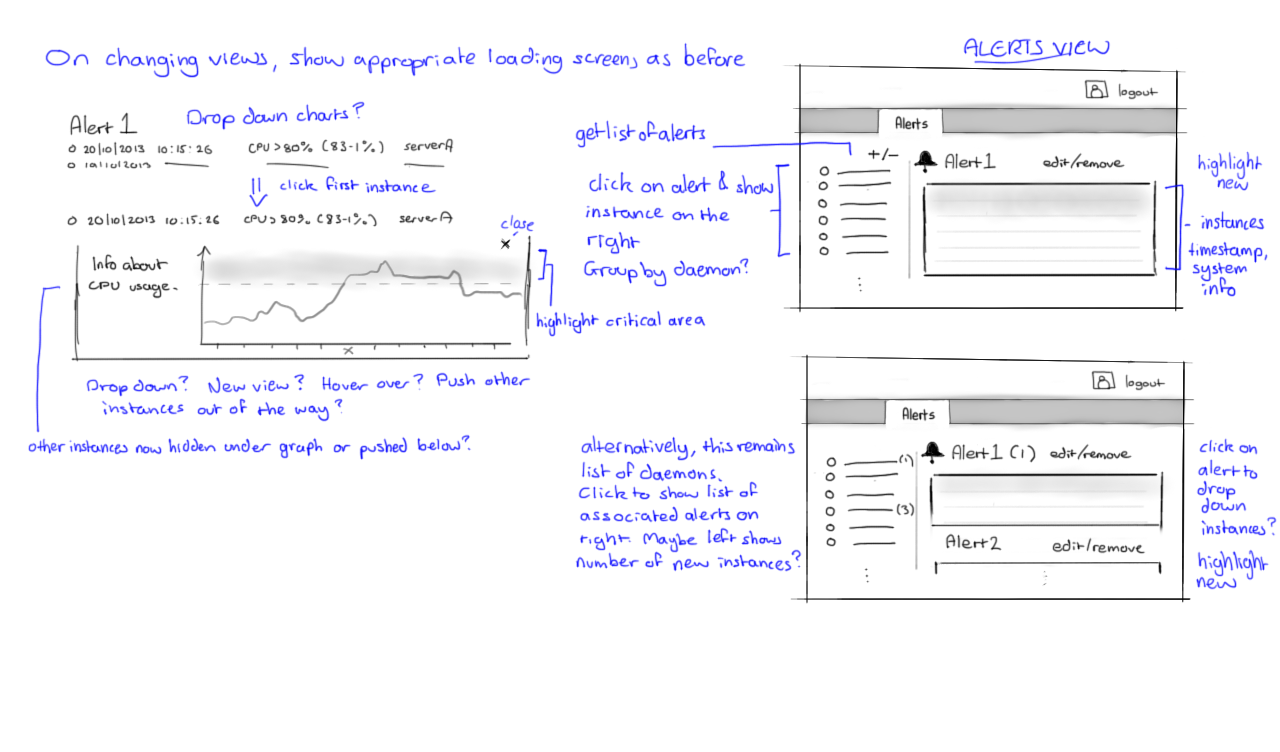
\includegraphics[width=110mm]{Concept_Designs/AlertView.png}
\caption{Alert View}
\label{fig:AlertView}
\end{figure}

As discussed in Section \ref{section:MarketResearch} concerning Market Research, the team thought it would be useful to provide user configurable alerts. Figure \ref{fig:AlertView} shows how such an interface might look like. This view houses a bit more complexity when it comes to development, as this is where a user would both see any instances of an alert having triggered as well as create new alerts.

Again, maintaining consistency, a daemon is selected from the sidebar and the content panel becomes a scrollable list of all the user-created alerts for this daemon. Underneath each alert, is each time the alert has been triggered, with new alerts that the user hasn't interacted with being highlighted so that they are instantly recognisable.

A more experimental design is shown in the top-left of Figure \ref{fig:AlertView}. Here, when a user clicks on an instance of an alert, a graph is instantly generated from, say, 30 minutes before the alert was triggered up to the current time. Essentially, this is a non-customisable, drop-down History view ala Figure ref{fig:HistoryView}. It is providing instant context for the user about how their machine was performing leading up to the alert being triggered, and how it has continued to perform since. This could be a very useful feature to users but it does add difficulty to our implementation.

\begin{figure}[H]
\centering
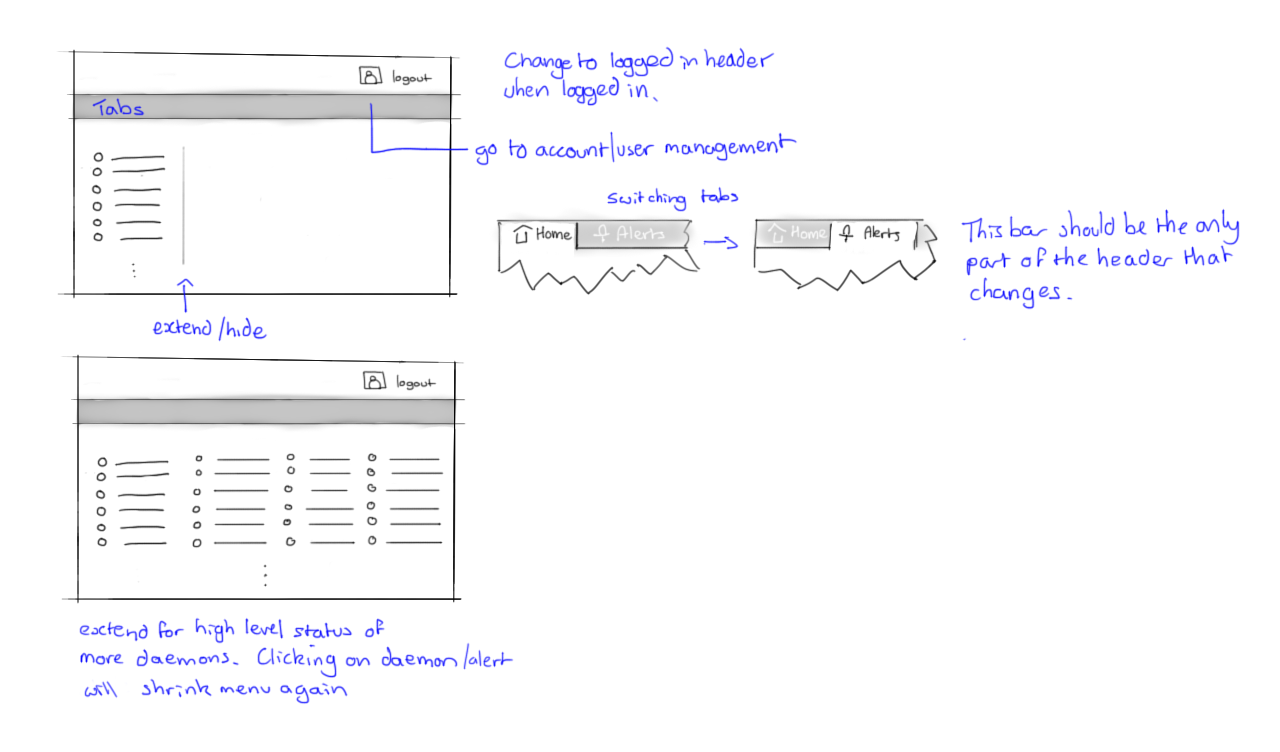
\includegraphics[width=110mm]{Concept_Designs/Misc.png}
\caption{Miscellaneous design features}
\label{fig:MiscDesign}
\end{figure}

Figure \ref{fig:MiscDesign} highlights some of the less feature-focused design considerations, such as the highlighted tabs being a way for the user to instantly know where they are in the application. Alongside this, it was considered that a user may have many, many daemons installed on multiple machines, so a small scrollable sidebar may not be useful all of the time. Hence, we designed a solution where the sidebar can be temporarily expanded to show a fullscreen list of daemons for the user to find the necessary daemon and select it, minimising the sidebar again. Here we also reiterate that this header is slightly different than when a user is logged out, showing user information, the option to logout, and the tabs.

%-----------------------------------------------------------------------------------------------------------------------------------------------

\section{Server}

\subsection{General overview}

\begin{figure}[H]
\centering
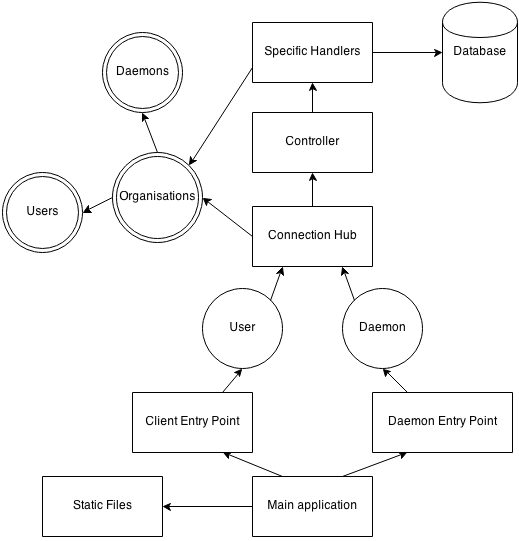
\includegraphics[width=110mm]{images/ServerDesign.png}
\caption{Design of the Server}
\label{fig:ServerDesign}
\end{figure}

(PROVIDE A KEY --- WHAT ARE THE ``TYPES'' FOR EACH SHAPE?\\BE CONSISTENT THROUGHOUT ALL DIAGRAMS)

While on first glance Figure \ref{fig:ServerDesign}, depicting the design of the server, might look very complicated, this is not really the case. Everything begins in the main application. This starts all the other parts, and this relationship is not shown to avoid cluttering the diagram. The main application registers handlers, tells (WHAT) how to serve static content, starts the connection hub and provides entry points for clients and daemons to connect to. Most of these things live in their own goroutines afterwards, and the main application just sits there, waiting for them to stop. In the following sections we will describe each of the components in the rough order of dataflow.

\subsection{Static content}

The main application sets up a file server that serves static content to the client. The client application itself is hosted here, being served together with all of its scripts and stylesheets.

\subsection{Entry points}

There are two entry points to this application, mapped to two different routes: `wsclient' and `wsdaemon'. Both of them are accessed via websockets and produce the same connection object that is to be handled by the connection hub. We need two separate handlers in order to attach an owner to those connections, because the application needs to differentiate between them. We show these connection objects as User and Daemon on the diagram, and they are being channeled to the hub via the register channel, in order to actually incorporate them into the application.

\subsection{Connections}

Connections are objects holding an open websocket, sending channel and an owner, which is either User or Daemon. There is a one-to-one relationship between owners and their connections. Once created, they result in two goroutines, one of which listens for the incomming messages and broadcasts them to the hub, and another sends messages back from the server to the client or daemon, depending on who created it.

(HAVE YOU DEFINED WHAT A GOROUTINE ACTUALLY IS? --- LIKE AN ACTIVATION/CALLBACK)

\subsection{Connection hub}

The connection hub serves three purposes, accomplished via three different channels. It accepts new connections on the register channel and stores them internally. It authorises these connections and adds them to the anonymous organisation (more about organisations later). It also deals with closing those connections and removing them from the application, when it receives such call on the unregister channel. Then it listens for the incoming messages from the currently open connections and forwards them to the controller. 

\subsection{Organisation}

The organisation is much like a namespace in the current design. It holds its own daemons and users, once they are authorised. It also provides a communication interface: all the daemons and users should only be accessed through the organisation object. It is a runtime tool – it only holds the currently active entries, however, it has its representation in the database, with which we can get all the users and daemons that belong to the given organisation. 

Authorisation, however, happens only after a certain request from the connection. Prior to that it lives in the anonymous organisation, a pre-created entity designed just for this use. While the connection belongs to that organisation, its reach is limited, as it can only execute handlers connected to proper authorisation.

\subsection{Controller}

The controller accepts json messages that are being sent by the connections, parses them, and executes their respective handlers, providing them with the message data. It knows which handler to use, because the main application has informed it of this by registering the handlers at the very beginning. When it fails to find one though, it returns an error message. Otherwise, it returns the result of the handler, which can be either an error object or null, so that the errors can be handled outside of the controller.

\subsection{Handlers}

Handlers implement a small piece of functionality associated with the particular API call. They are being registered by the main application, and invoked by the Controller, upon receiving the aforementioned call. They are being given an already parsed request as opposed to serialised json, and it is their responsibility to check whether the call adheres to the API, including the typechecks. Handlers return error objects for the errors they might encounter, which are then sent back to the requester from the hub as a special error message. In the case of a success, they themselves send the result messages, if any, to the connections involved.

\subsection{Database}

Using a NoSQL database (MongoDB) turned out to be a real challenge, since the principles of its design differ significantly from the relational databases that we were used to. While in the relational database one generally tries to achieve third normal form, in the NoSQL database one tries to denormalise data in order to match the usage pattern. Hence, we have identified two potential approaches to the problem: we could either design the database in a way that is easy to use for us and then provide the user with means of interaction, or we could devise the most sensible usage patterns and then adopt the schema to suit these needs. Being customer-centric, we have decided to stick with the latter option.

Hence, we have come up with the following database schema:

\begin{figure}[H]
\centering
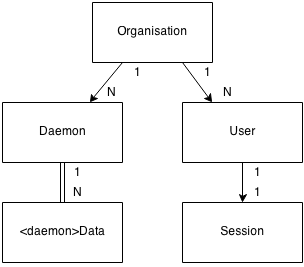
\includegraphics[width=80mm]{images/DatabaseSchema.png}
\caption{Database Schema}
\end{figure}

The diagram is self-explanatory end looks vaguely familiar, but there is one NoSQL feat in this schema. Most of the relations are done in the regular fashion: Organisation has many Daemons and many Users, each User has one Session. Each daemon has many data points attached to it, and this is implemented in an unusual way – instead of having a foreign key that references the Daemon table, as we would do in a relational database, each daemon creates its own collection that has a name based on the daemon's name. MongoDB supports lots of collections in its namespace, so this allows us an efficient way to retrieve the data now that it is always available from the same daemon in one collection. In such a way we optimise for our usage pattern, since the user will usually want to see a piece of history from one given daemon.

%-----------------------------------------------------------------------------------------------------------------------------------------------

\section{Daemon}

\subsection{Overview}

The daemon's two most important parts are the watchers, which gather the information about the different parameters that are being monitored, and the connections, which communicate back and forth with the server and connected clients. A central manager handles them and ties them together.

\subsection{Watchers}

Each watcher is associated with one parameter that the daemon monitors. Currently, the watchers are:
\begin{itemize}
  \item CPU, which reports the overall utilization of the CPU as a percentage
  \item RAM, which reports the overall RAM utilization in bytes
  \item Network, which reports the total upstream and downstream added up, in bytes/second
\end{itemize}
These watchers are templates for platform-specific implementations, and are used by the central manager to get data in the same format without needing to worry about the platform the daemon is running on after the watchers have been created and started.
Generally, the structure of each watcher is similar: they begin running in parallel, getting the desired parameter every few seconds, according to the refresh rate they were set to, and they offer a way for the manager to retrieve the data resulting from that operation.

\subsection{Connections}
There are two asynchronous connection managers. The first one opens the connection to the main server, and allows any data to be sent to it from the main daemon manager, and the second accepts any number of connections from clients, and can simultaneously send data to all connected clients through the main manager.

\subsection{Manager}
The component that initializes and ties everything together. It synchronizes the refresh rates of the watchers, and sends messages to the server and clients through the connections.

%===============================================================================================================================================

%===============================================================================================================================================

\chapter{Implementation}
\label{impl}

In this chapter, we describe the low level details of how the high level designs discussed in the previous chapters were used to construct our product.

%-----------------------------------------------------------------------------------------------------------------------------------------------

\section{Initial Steps \& Coordination}

\subsection{Team Organisation}

At the beginning of the project we thought that we would have a laissez faire approach to development within our team, however, soon some specific roles formed within it, influenced by the very modular design of the whole system. We had one person driving the design and helping with the client side, one person working on a client side solely, one person working on the server side, one person working on daemons, and finally one person on the user manual duty. These roles then stayed for the duration of the whole project.

We would usually have three formal weekly meetings in our team: on Tuesdays to drive the development, on Thursdays with the supervisor to catch up on what was done and ensure that we are on track, and straight after that yet another short team meeting to address the supervisors feedback. Meetings were the place where most of the decisions would have been made, thus they were extremely important to the whole development process.

In addition to that, we have used plenty of other communication media. We had a facebook group where we would post current headlines. During the intensive phases of the development process we would use skype conference calls if we were working remotely. In order to keep track of current issues we had a Kanban board online. Finally, we had exchanged our phone numbers with each other so that we could be contacted directly in case of emergency.

\subsection{Developing an API}

The first and most important step was

\subsection{Technology Prototypes}

% Our first attempts at creating a simple echo server, getting all the components to talk to each other...

ALEX

GABRIEL

MAKSIM

%-----------------------------------------------------------------------------------------------------------------------------------------------

\section{Implementation Of The Client Application}

\subsection{User Interface}

User interface implementation is fully based on the approaches provided by Backbone.js framework. Every logical part of the UI is implemented as an independent Backbone model and a corresponding view. For example, a daemon is an extended Backbone model that implements a high level of daemon abstraction. It has some methods for controlling the daemon (starting, stopping, changing the metrics to monitor, etc). All the daemons are stored in a standard Backbone Collection. There is a View definition that is implemented as a Marionette ItemView that controls the way a single daemon is rendered on the page. The rendering is done by creating a template which describes what information has to be shown to the user. Also, the ItemView contains some event listeners that implement the processing of user actions (such as selection). Finally, there is a CompositeView (which is a part of Marionette) that describes how the whole collection of daemons is rendered. It has a template as well.

The same approach is used with tabs and charts.

\begin{figure}[H]
\centering
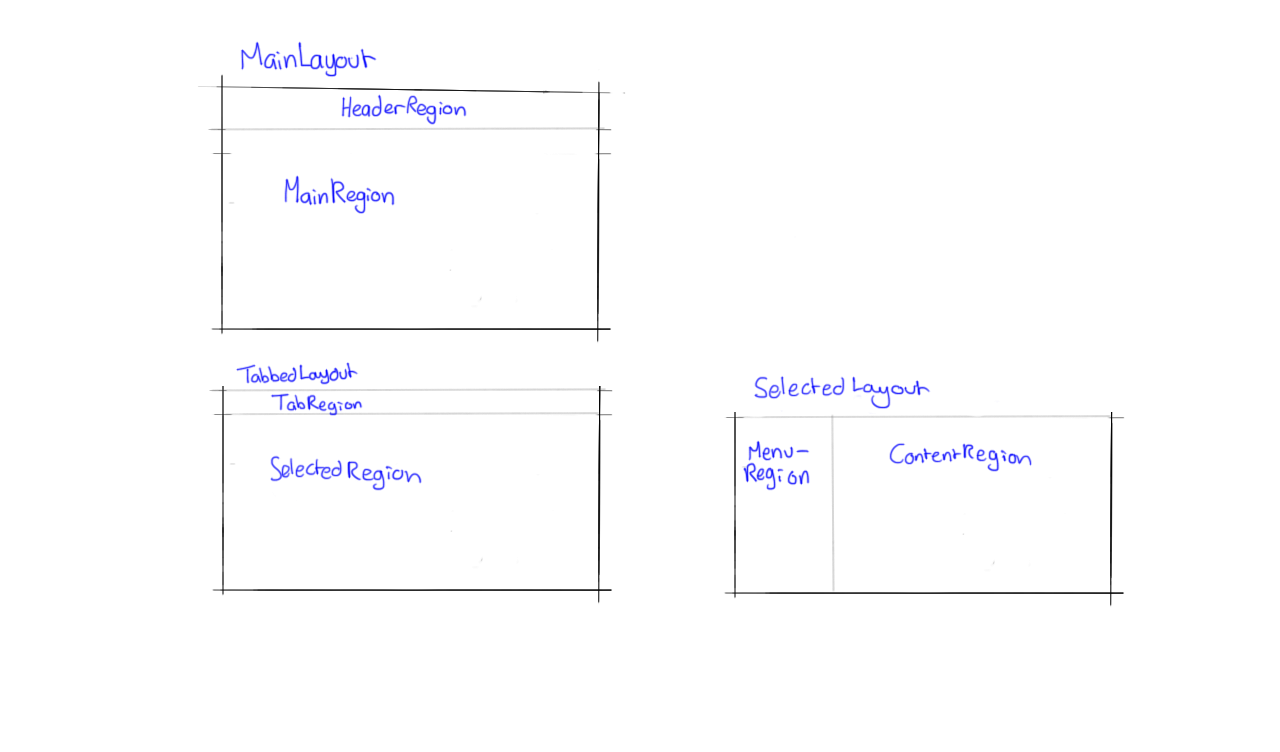
\includegraphics[width=110mm]{Concept_Designs/BackboneLayouts.png}
\caption{Backbone Layouts}
\label{fig:BackboneLayouts}
\end{figure}

In order to try and simplify the process of translating the concept designs to code, some templates were discussed that could be directly mapped onto Backbone's own templates. Figure \ref{fig:BackboneLayouts} shows these layouts, and also highlights how our design aims for consistency as much as possible, with switching tabs changing at most two regions, the ContentRegion and MenuRegion.

The example of code is shown below.

Actually, do we have to show the examples of code? It can take A LOT of space.

(CAN PUT IN APPENDIX, OR GIVE PSEUDO-CODE IF YOU HAVE ANY INTERESTING ALGORITHMS)

\subsection{Communication}

One of the most important parts of the application is the communication component. It consists of the definitions of all the types of the messages (which includes the data format and the callbacks for all types of requests), the message parser and validator. Every incoming/outcoming message is checked to be well-formatted before processing/sending. (MORE DETAILS) On an event of receiving a well-formatted message it is processed by an appropriate callback function which does the low-level data manipulations and then passes control to a higher level listeners and processors. For example, if the user wants to send a "control" message to the server (the message specifies the id of controlled daemon and the action) the following things happen:
\begin{itemize}
  \item The message is created by a message processor which accepts the message type and its data, packs it into a JSON object, validates and returns it.
  \item The message is passed to the server's websocket send function that send it using the native approach.
  \item The client has to wait for the response. In some cases it may not be instant.
  \item When the response iS received, the incoming message is parsed and checked to be valid.
  \item The control is given the callbacks that evaluate the answer and undertake the corresponding actions.
\end{itemize}

\subsection{Sockets}

There are two types of sockets in the client application. The first one is the ServerSocket. It implements the interface provided by the standard WebSocket object. It is used as is without any wrappers. The second type is the DaemonSocket. It is implemented in the same manner as the first one except it has a bi-directional link with a corresponding daemon (which means that it "lives" inside the Daemon object and is meaningless without it). This socket also can be used to send data but this functionality is not used as our design assumes that all the client-daemon messages have to be deligated to the server. This improves the consistency of the states.

\subsection{Charts}

(GIVE SCREENSHOTS)

Charts are drawn on the HTML5 canvases that are passed as parameters for the Chart.js chart constructor. Each chart is capable of showing a history of a custom length. For real-time charts this is 20 points. For the history this value varies heavily as it depends on the data period selected.

Generally, there is a class called Graph which implements an abstract chart. There are classes for cpu, hdd, net and ram charts that extend the functionality of the base class. On every incoming "monitoring" message the graphs are updated.

\subsection{States}

(USE TELETYPE FONT /\ texttt FOR CODE ENTITIES WHEN YOU DESCRIBE THEM)

The components of the application and their different view should use shared data (for example, the current daemon). This could be done by introducing a number of global variables. Backbone offers a better approach. In our case an instance of AppState model is responsible for storing all the shared data. It does not only store the information, it is also responsible for listening to the change of the data and firing all the necessary updates. For example, when the user logs in, the is user "logged in flag" is set to true in the controller. This event is immediately caught by an according listener and the current view changes. Here another component comes to the action and it is called Router.

\subsection{Routing}

Router is a standard method for handling the routes. In the use case described above, the Router's method ``navigate" is called. The AppState's listener passes the name of the page that has to be shown and two things happen. Firstly, routes changes the hash of the window's location object. This change is added to the history stack so the user is able to use the history object (which implies an opportunity of browsing the application using back and forward buttons). This also guarantees that the page can be bookmarked. Secondly, the Router executes a callback that is associated with the name of the requested page. In our case, when a user requests for the "app" page, the AppState's variable called "current state layout" is set to the new value. Here AppState's listeners again start doing their job - as the value has changed, an according action is performed - the page layout is set to the app's home view. Routing, together with objects like AppState, are extremely efficient in dealing with routing and shared data.

\subsection{Service}

There is a service component that provide some helper methods for working with cookies and some other things.


\subsection{Problems During Development}

(DEALING WITH UNFORSEEN CHALLENGES IS A \textbf{KEY} PART OF A GOOD PROJECT --- EMPHASISE YOUR CHALLENGES \& SOLUTIONS)

The probles will be described here. (Struggling with Backbone, choosing the framework for charts, testing, data simulation when no actual daemon is available, etc)

\subsection{Stability}

Client-server connection restores if lost.
Client-daemon connection restores if lost in absolutely the same manner as this is done with the client-server connection.
-- notfinished

\subsection{Testing}

The most important part that has to be tested is the communication. This is done by creating some custom messages for each type of message. The answer is checked to be valid.
-- notfinished

%-----------------------------------------------------------------------------------------------------------------------------------------------

\section{Implementation of the Server side}

\subsection{Creating an echo server}

One of the first steps in building a server was to test how it handles websockets and using them integrates with client and daemon. We have taken an echo server as a good starting point, and modified it, so that it accepts and differentiates between users and daemons. It would simply retranslate messages to everyone connected, however it had means of directing the flow specifically to daemons or users, or to stop echoing back. We have connected it to the initial implementations of users and clients and in this way we got assured, that the tri-way websocket connections will work. Knowing that we have proceeded to the next development stages.

\subsection{Developing tools for testing}

We were developing three different parts to the whole system in parallel, and the development speed would vary, so we needed some tools to ensure that the server actually works. We have decided to take the TDD approach in developing it, because Go was an unfamilliar language and every little indication that what we were writing made sense would have helped us greatly.

Go comes with a testing framework, not unlike JUnit, out of box. It is implemented in the spirit of table testing, but table testing was of little help in this application. The application mostly communicates via messages and changes its internal state, so an enhanced ability to stub things would have helped. Unfortunately, Go lacked of this ability, thus we had to create workarounds, mostly consisting of altering the real application state to create a specific environment, and then restoring it back to pre-test condition. We have devised ways to insert temporary objects into the database, create stub handlers, and interceipt sent messages during the testing. All of this allowed us to introduce acceptable levels of testing.

One controversary addition to the test harness was the Assert() method, that would abstract away the clumsiness of Go test framework and provide rspec/jasmine style coloured output. We felt that colour-coding success and failure messages in the test harness made the whole process more robust, (THIS SEEMS A TRIVIAL POINT TO ME!) however abstracting away Log() and Error() calls meant that the test harness could no longer tell on which line did the error occured. It was still fine, knowing that every single Assert() message was unique-ish; nonetheless, if we had substantially more test cases this drawback might have slowed us down.

Yet another issue was that we could not separate away test files from the main code, because that would have created some probles with namespaces. We could not resolve it at the time and we have felt that this made the sourcecode less clean, but this is more of an annoyance than a real problem.

Overall, introducing tests was a great success. Go extremely fast compilation speed and performant testing framework allowed us to run tests before each deployment, and we have written scripts to do so. As a result of TDD we have a fair test coverage, (CAN YOU QUANTIFY IT?) and the integration process with the rest of the codebase was indeed relatively painless.

\subsection{Creating the controller}

We have decided that handler pattern would be the most suitable for our needs. The different API calls seemed to be quite independent from each other semantically (while sometimes required to be called in a particular order), and their list was by no means final. Having means to register handlers allowed us to be extremely flexible on the development of them.

The Controller part was re;latively simple to write, since it turned out to be extremely testable. Being able to write comprehensive tests, we could develop it relatively quickly, rapidly fixing any arising problems. 

\subsection{Implementing each separate handler}

Each handler was developed separately. The most problems have arisen due to Go being a strongly typed language, while JavaScript, that was producing json requests, is not, and hence it was sometimes difficult to parse the message into correct types. In fact, this error was so common, that we had to abandon idealogically unit tests and expand them to cover parsing from actual json (which was tested in the Controller and was definitely working), for the parsed result was sometimes now what we would have expected.

Aside from that another problem of handlers is that there is a lot of boring typecheck code in them, there should have been a way to avoid this. Possible solution would be to move that code away, creating a type of framework for even fuller parsing of requests. However, due to the time constrains we have decided to skip this improvement for now.

%-----------------------------------------------------------------------------------------------------------------------------------------------

\section{Implementation of the Daemon}

\subsection{General}

In order to satisfy our requirements for performance, stability, and multi-platform compatibility, the daemon is written in C++, using features of C++11 as well as the Boost library for threading and as a requirement to the websockets library used, WebSocket++.
C++11 provides many new features, allowing us to both simplify parts of the code as well as use complex features, mostly through WebSocket++. In order to work with these libraries as well as C++11, Microsoft Visual Studio 2012 was used to program and compile the project under Windows, and GCC/G++ 4.8.2 was used under Linux, along with the full Boost libraries version 1.54.0 and WebSocket++ 0.3.0-alpha4.

\subsection{Manager}

The main manager begins by including all the abstract watchers, and then using preprocessor checks in order to detect the platform on which the daemon is being compiled, in order to include the platform-specific watcher code, as well as initialize the watchers. The client and server connection managers are also included, then initialized. A new thread is created for each of them, in which they can run and both listen for and send messages. 

During initialization, the manager makes the server connection start communication with the server by sending a login message, which containts the name of the daemon, a password, and an ID that can identify the user/organization. The server connection is also bound to a message handling function inside the manager, which will receive any message from the server in order to parse it and take the necessary actions.

After connection initialization, the watchers are started, and their status is updated in a map, so the daemon can track which watchers should send data. When all the watchers have started, the manager begins a loop, in which the manager gathers data from the watchers and sends it in our standard format to both the server and any connected clients, through the connection managers, every few seconds, with a refresh rate synchronized to that of the watchers themselves.

\subsection{Server connection}

Implemented as a simple asynchronous websockets client, the server conection manager uses four handlers, the most important ones being the send handler, which simply sends a string payload to the open server connection, and the receive handler, which is tied to a callback to the main manager, sending any messages received from the server to it.

\subsection{Client connection}

Implemented as a asynchronous websockets server, the client connection manager uses handlers that are similar to the server cconnection manager's, but due to the fact that it must support any number of clients, it saves new connections in a set when they are open, and removes them from the set when they are closed. The send message handler is similar as well, but it iterates through the client set and sends the given message to every connected client. There is a message handler implemented to display any message a client might send, but these are not parsed in any way, as our protocol does not define any valid messages that a client can send to a daemon directly, all messages having to go through the server.

\subsection{Watchers}

The watcher for each parameter is implemented as "abstract" class, with all of them having simlar methods - in the future they could be refactor to all inherit from one abstract watcher class. All of them hold a refresh rate time, in milliseconds, offer functions that start the watcher, get the latest usage statistic, and update this usage statistic - to be used from within the platform-specific watcher implementation. Every watcher is based on a loop function, that works with either a default refresh rate or one provided when the watcher is initialized, and runs in a thread.
Every watcher is only compiled if the platform the daemon is being compiled on matches its platform. This is done by setting an exclude from build flag in Visual Studio, and not including the file in the Makefile in linux.

\subsubsection{CPU Watcher - Linux}

The linux CPU watcher bases its loop on parsing data from the first line of "/proc/stat", which contains information about how many total CPU cycles there have been since the machine turned on, and how many of those were in use for different purposes. The watcher gets these values and saves them, adding up the used cycles, then doing the same on the next refresh and subtracting the old data from the newest one, getting the total number of cycles elapsed since the last refresh, and how many were used of those. By dividing the used ones by the total ones and multiplying the result by 100, the watcher can update its usage with that number, representing the total CPU usage in percentage over that time.
A CPUCycles class is used to more easily organize the number of used and total cycles. The watcher holds two instances of this class, in order to hold the cycle information for both the current and the last parsing cycle, which are used to calculate the precentage usage.

\subsubsection{CPU Watcher - Windows}

The Windows CPU watcher is based on querying performance counters using the PDH interface - a windows specific interface that can access a very high number of performance counters which are maintained by the operating system. Because of this, the code is simpler than the linux watcher - to start the watcher, the correct query for total processor usage is added as a PDH counter, then the loop is started which collects data for this query every few seconds based on the given refresh rate, updating the usage variable with it.

\subsubsection{RAM Watcher - Linux}

Linux standard libraries offer a sysinfo structure, which holds a few useful parameters, including total and free memory amounts. As such, the linux memory watcher uses this directly to get the amount of used memory, by subtracting free memory from total memory, and update its usage variable with every refresh cycle. It also offers a function that returns the total memory available on the machine, which simply returns the total memory as reported by the sysinfo structure.

\subsubsection{RAM Watcher - Windows}

Windows provides a similar standard structure to linux for memory data, called MEMORYSTATUSEX. This struct is checked on each refresh cycle, and the total and available memory are retrieved from it, then used to uptade the usage through subtraction. A total memory function is also provided, which simply retrieves the total memory from this structure and returns it.

\subsubsection{Network Watcher - Windows}

The network watcher implementation on windows uses the PDH interface in a similar way to the CPU watcher. To start the watcher, a query is created that can retrieve the total bytes per second from the first network adapter. This is then used on every refresh cycle to update the usage variable.

%===============================================================================================================================================

%===============================================================================================================================================

\chapter{Evaluation}

(DO THIS)

We evaluated the project by...

%-----------------------------------------------------------------------------------------------------------------------------------------------

\section{First Client Feedback}

Our first visit to J.P Morgan

\section{Final Client Feedback}

TBD

%-----------------------------------------------------------------------------------------------------------------------------------------------

\section{Daemon performance testing}

%-----------------------------------------------------------------------------------------------------------------------------------------------

\section{Server load testing}

We have reused the capabilities of our testing framework to create a working environment with thousands of users, hundreds of organisations and tens of thousands of daemons. To do so, we have written a testing application that is capable of dispatching multiple requests cuncurrently. The benchmark of success was how many people will it correctly serve.

%===============================================================================================================================================

%===============================================================================================================================================

\chapter{Conclusion}

We da bomb!

%-----------------------------------------------------------------------------------------------------------------------------------------------

\section{Summary}

%-----------------------------------------------------------------------------------------------------------------------------------------------

\section{Future Work}

Implementation of Alerts

Maksim's server stuff

More metrics to monitor?

%-----------------------------------------------------------------------------------------------------------------------------------------------

\section{Contributions}

Here we explain that Sean Jakobsen coordinated the rdissertation writing, conducted market research, drew the design prototypes and worked on the client application. 

Maksim Solovjov conducted market research, liasoned with our clients at J.P Morgan and wrote the Go server and database components.

Aleksandrs Sidlovskis drew up our architectural diagram and worked heavily on the client application.

Gabriel Alexandru Susanu developed the platform-specific daemons and their ability to monitor the different metrics needed.

Supanat Auengsirirat wrote our help manual and assisted with some daemon functionality.

%===============================================================================================================================================

%===============================================================================================================================================

\bibliographystyle{plain}
\bibliography{example}
\end{document}